\documentclass[10pt,a4paper]{report}
\usepackage[style=numeric, backend=biber]{biblatex}
% Packages for formatting and styling
\usepackage{graphicx} % For including images
\usepackage{hyperref} % For hyperlinks and metadata
\usepackage{fancyhdr} % For headers and footers
\usepackage{geometry} % Adjusting page geometry
\usepackage{lastpage}
\usepackage{tabularx}
% Page geometry
\geometry{
    a4paper,
    top=2.5cm,
    bottom=2.5cm,
    left=2.5cm,
    right=2.5cm
}
\usepackage{float}

% Define variables
\newcommand{\delivtitle}{D4.1 -NGSOTI architecture document}
\newcommand{\delivdate}{23 September 2025}

% Hyperref setup
\hypersetup{
    pdftitle={\delivtitle},
    pdfauthor={TEAM NGSOTI},
    pdfsubject={EU Project Deliverable Report},
    pdfkeywords={NGSOTI, EU Project, Deliverable, Cybersecurity},
    colorlinks=true,
    linkcolor=blue,
    urlcolor=blue
}

% Set up the header and footer
\pagestyle{fancy}
\fancyhf{} % Clear all header and footer fields
\fancyhead[L]{NGSOTI – Project: 101127921 —  DIGITAL-ECCC-2022-CYBER-03}
\fancyfoot[C]{\delivtitle{} - Page \thepage/\pageref{LastPage}}

% Title page setup
\title{
    \Huge \textbf{\delivtitle} \\[0.5cm]
    
\includegraphics[width=0.3\textwidth]{img/ngsoti.eps}
    \hspace{1cm}
    
\includegraphics[width=0.3\textwidth]{img/eu_funded_en.eps}
}
\author{\textbf{TEAM NGSOTI}}

\date{\delivdate}
%\addbibresource{ngsoti-deliverable-4.1}
\addbibresource{ngsoti-deliverable-4.1.bib}
% Document starts here
\begin{document}


% Title page
\maketitle
\thispagestyle{empty} % Remove header and footer from the title page

% Table of contents
\newpage
\tableofcontents
\newpage
\section*{Disclaimer}
Co-funded by the European Union. Views and opinions expressed are however
those of the author(s) only and do not necessarily reflect those of the
European Union or the European Cybersecurity Competence Centre. Neither the
European Union nor the granting authority can be held responsible for them.
% Main content

\section*{Deliverable definition}
The identifier of the deliverable is \textbf{D4.1} and it adheres to the
definition outlined in the grant agreement written in \textbf{bold}.
\textbf{Blog post of the NGSOTI architecture and exploitation  to collect data
on d4-project.org}.

\section*{Executive Summary}
\addcontentsline{toc}{section}{Executive Summary}

The blog post was published on \url{https://d4-project.org/2025/06/19/NGSOTI-Architecture-Overview.html}
and is accessible via the above link.
The content is included in this deliverable.


\chapter{NGSOTI – Architecture Overview}
The Next Generation SOC Training Infrastructure (NGSOTI) project\cite{ngsoti}
is an open-source initiative to build realistic, reproducible SOC
environments for training and education. It integrates mature open-source
components with \textbf{ReST APIs and OpenAPI specifications} to ensure
interoperability, scalability, and extensibility.

This document aims to present a comprehensive overview of the
NGSOTI architecture while also reflecting on the insights, feedback, and
experience gained during the initial phase of the project.

\begin{figure}[h]
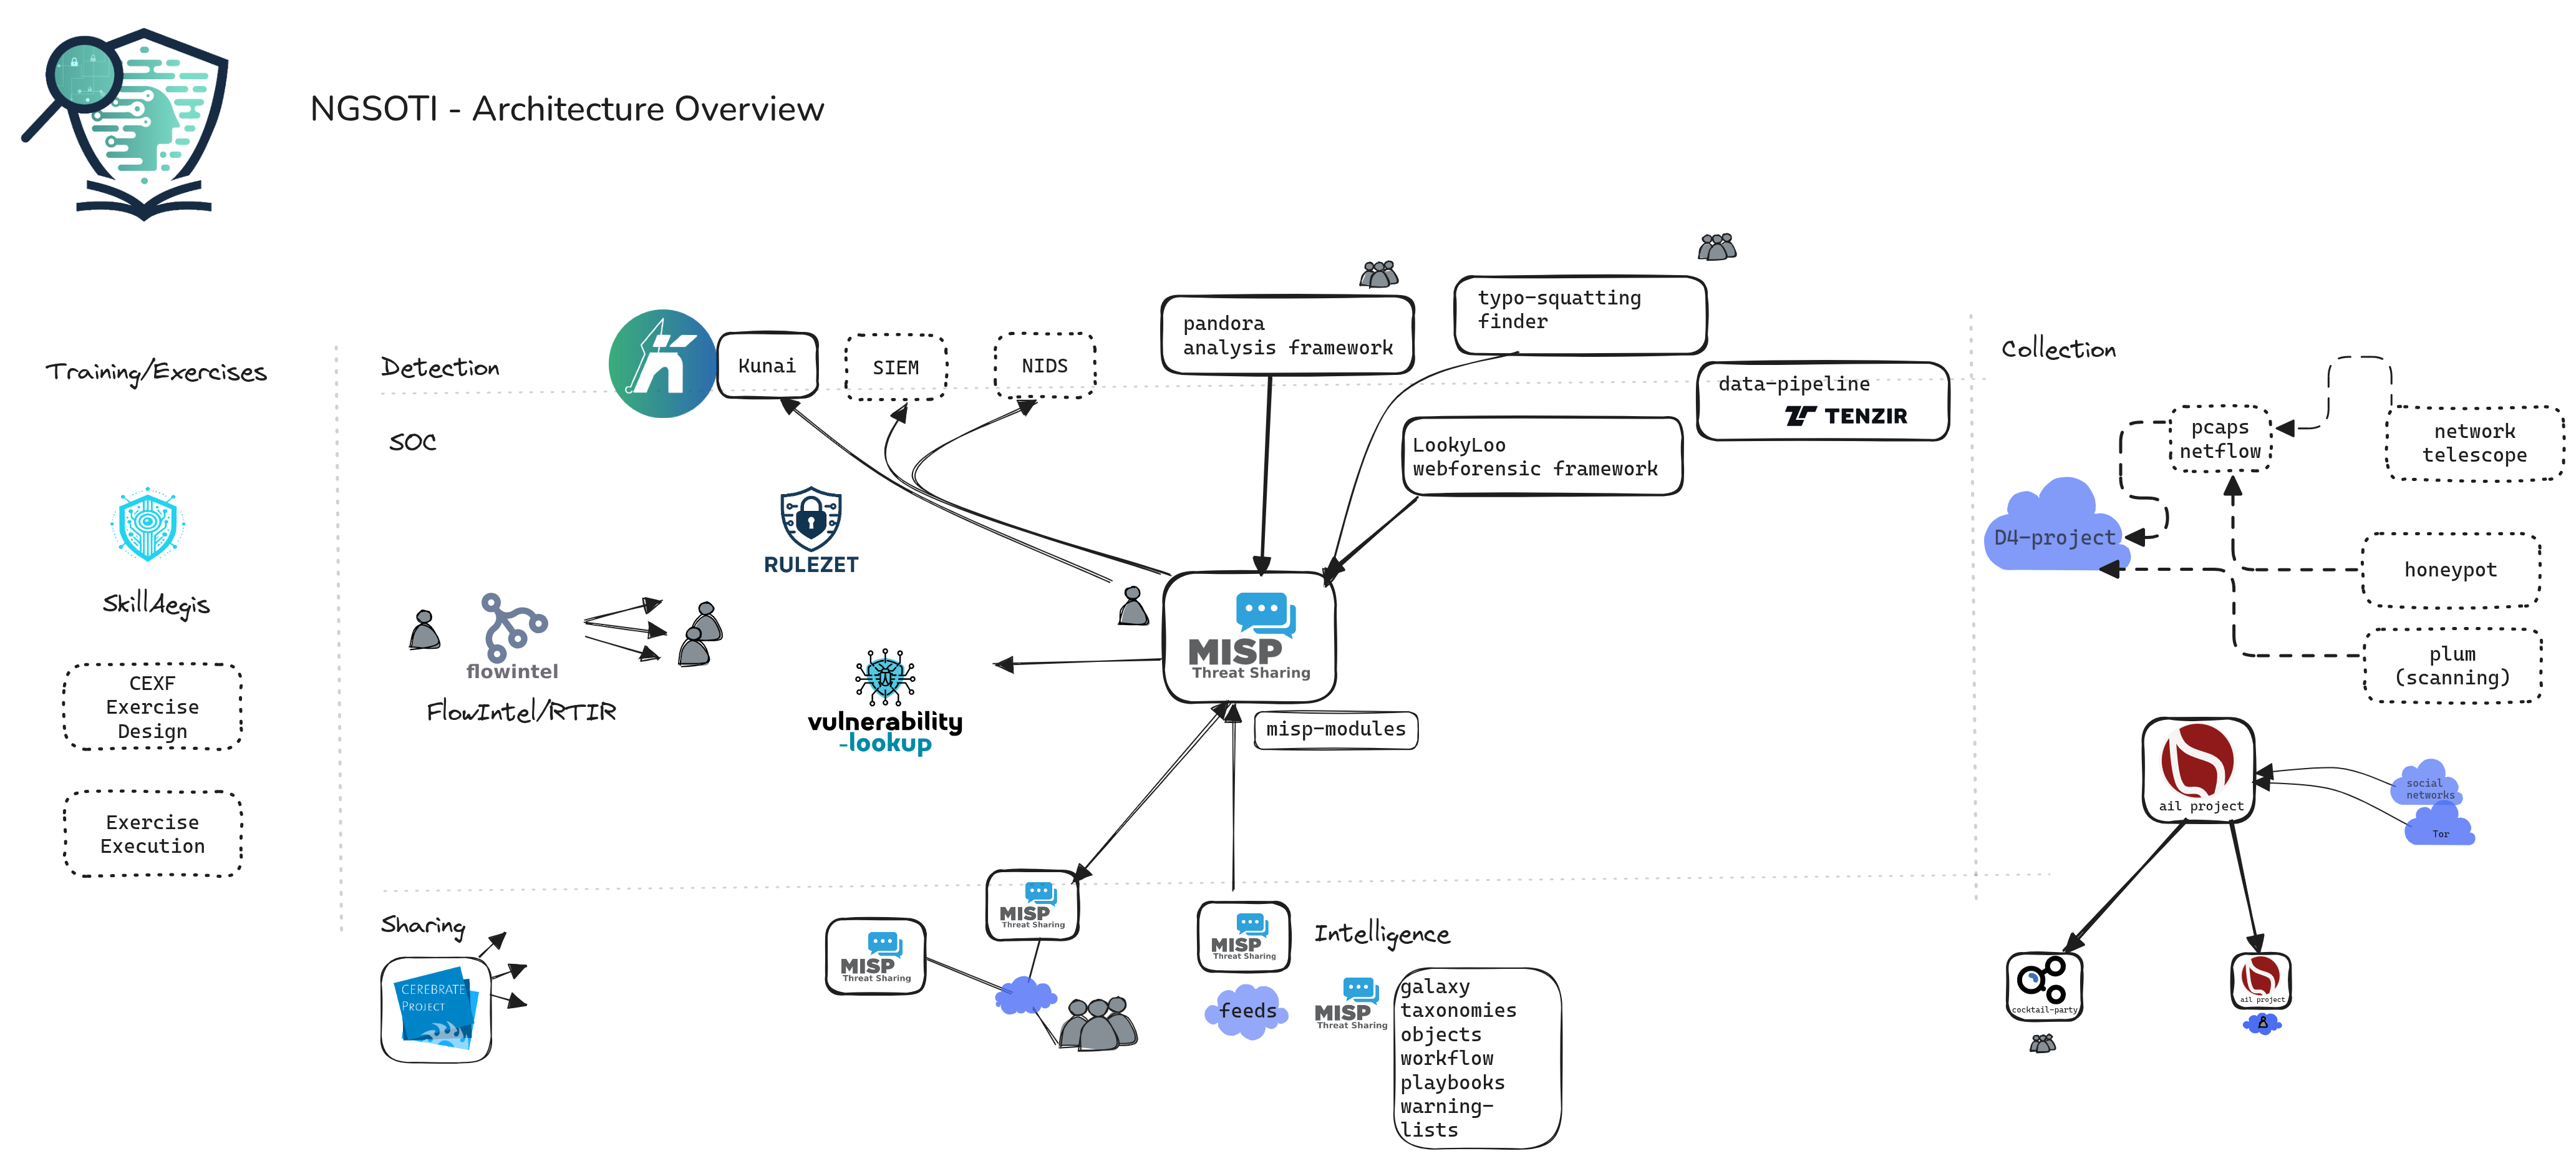
\includegraphics[scale=0.11]{oss-overview.png}
\end{figure}

\section{Scope}

The NGSOTI project is designed to replicate the day-to-day environment of a
modern Security Operations Center (SOC) and provide trainees with the
essential skills required to operate effectively in such settings. To achieve
this, the training infrastructure must cover the core requirements of SOC
analysts and incident responders:

\begin{description}
    \item [Log Management and Analysis] SOC analysts must be able to collect,
          normalise, store, and query large volumes of heterogeneous logs
          (endpoint, network, application, cloud). Training scenarios need
          to expose students to real log pipelines, from raw ingestion to
          search and correlation.
    \item [ False-Positive Handling and Triage ] Analysts must learn to
          distinguish between benign anomalies and true security incidents.
          Training must include workflows for alert triage, suppression of
          recurring false positives, and case escalation.
    \item [Detection Engineering] SOC teams are not only consumers of alerts
          but also creators of new detection rules. Training requires
          environments where students can experiment with creating, testing,
          and deploying new signatures, queries, or behavioural detections
          across different telemetry sources.
    \item [Information Sharing and Collaboration] Modern SOCs rarely work in
          isolation. They rely on information exchange with other teams and
          communities. Exercises must therefore include mechanisms for sharing
          Indicators of Compromise (IOCs), Tactics, Techniques, and
          Procedures (TTPs), and incident reports in structured formats.
    \item [Threat Intelligence Integration] To contextualise alerts and drive
          better decision-making, analysts need access to threat intelligence
          feeds and vulnerability information. Training environments must
          integrate open-source threat intelligence platforms (e.g., MISP) and
          vulnerability knowledge bases (e.g., Vulnerability-Lookup) to provide
          authentic enrichment and prioritisation workflows.
\end{description}


By embedding these requirements into the training scope, NGSOTI ensures that
students are not only exposed to realistic datasets and tools, but also to
the \textbf{operational processes} and \textbf{analytical workflows} that
define real-world SOC operations.
This explains the architectural choices described in the following sections.

\section{Purpose of the Architecture}

NGSOTI addresses key challenges in SOC training:

\begin{description}
    \item [Infrastructure Access:] Many training centers/universities lack
          resources to simulate SOC environments.
    \item [Integration with Modern Tooling:] SOC tools evolve quickly; training
          must adapt.
    \item [Reusable Exercises:] Scenarios must be standardised (via CEXF) for
          replay and sharing.
    \item [Accessible Datasets:] Trainees should work with realistic telemetry
          and dataset from real-world sources.
\end{description}

\section{Layered Design}

\begin{table}[h!]
\centering
\begin{tabularx}{\textwidth}{|l|X|}
\hline
\textbf{Layer} & \textbf{Components} \\
\hline
Trainee \& Instructor & SkillAegis \\
\hline
Telemetry & Kunai, Zeek, Suricata, Sysmon \\
\hline
Data Pipeline & Tenzir, Poppy \\
\hline
Threat \& Vulnerability Intelligence & MISP, Vulnerability-Lookup \\
\hline
Collection & D4 Project, Honeypots, Network Telescope \\
\hline
Storage & NFS, S3 / MinIO \\
\hline
Analyst Tooling & FlowIntel, RTIR, Wazuh dashboards \\
\hline
Dark Web \& OSINT & AIL \\
\hline
Forensics \& Enrichment & Lookyloo, Typo-squatting finder, Pandora \\
\hline
Sharing & Cerebrate \\
\hline
\end{tabularx}
\caption{Overview of layers and their associated components}
\label{tab:layers-components}
\end{table}

\section{Component Details}

It is important to note that the components described in this section
represent the \textbf{current set of integrated tools}, but the architecture is
not limited to these specific projects. The NGSOTI stack is intentionally
designed to be \textbf{modular and extensible}, making it possible to replace,
extend, or complement components as new tools and technologies emerge. This
means that future iterations of the architecture document can evolve to
incorporate additional open-source projects, new detection capabilities, or
alternative analyst platforms, while still adhering to the same design
principles of interoperability, open standards, and reproducibility.

\subsection{SkillAegis \& CEXF}
\begin{description}
  \item[Purpose:] Web portal for instructors and trainees. Defines and executes
        exercises in \textbf{Common Exercise Format (CEXF)\cite{cexf}}. Provides live
        scoreboard and feedback.
  \item[Inputs:] Exercise definitions (JSON), datasets, injects.
  \item[Outputs:] Exercise deployment instructions, scoreboard updates.
  \item[APIs:] ReST API (OpenAPI).
    \begin{itemize}
        \item ReST API (OpenAPI)
    \end{itemize}
  \item[Integration:] Pulls case status from FlowIntel, IOC/CVE
artefacts from MISP, and telemetry triggers from Tenzir.
\end{description}


\subsection{Kunai}

\begin{description}
  \item[Purpose:] Lightweight Linux sensor using \textbf{eBPF} for syscall and
       network visibility.
  \item[Inputs:] Kernel-level telemetry.
  \item[Outputs:] JSON structured logs (syscalls, processes, sockets, files).
  \item[APIs:] gRPC \& ReST endpoints to push events into pipelines. Online
       sandbox available at \url{https://sandbox.kunai.rocks/}.
  \item[Integration:] Feeds events directly into Tenzir for enrichment and
       storage or MISP event.
\end{description}

\subsection{Zeek}
\begin{description}
  \item[Purpose:] Network traffic analysis framework for metadata-rich logs.
  \item[Inputs:] PCAPs, live network traffic.
  \item[Outputs:] Connection logs, DNS, HTTP, SSL/TLS metadata in structured
  log format.
  \item[APIs:] Exposes logs via file or ReST exporter plugins.
  \item[Integration:] Tenzir ingests Zeek logs for correlation and enrichment.
  Integration with MISP.
\end{description}


\subsection{Suricata}
\begin{description}
  \item[Purpose:] IDS/IPS engine with signature-based traffic inspection.
  \item[Inputs:] PCAPs, live network traffic.
  \item[Outputs:] Alerts, flow records, protocol metadata (EVE JSON).
  \item[APIs:] Native EVE JSON output; ReST management API.
  \item[Integration:] Suricata alerts streamed into Tenzir $\rightarrow$
  Wazuh dashboards. Integration with MISP and also SkillAegis.
\end{description}

\subsection{Sysmon}
\begin{description}
  \item[Purpose:] Endpoint monitoring on Windows. Provides detailed process,
  file, and registry telemetry.
  \item[Inputs:] Windows system events.
  \item[Outputs:] XML/EVTX logs $\rightarrow$ converted into JSON.
  \item[Integration:] Shipped to Tenzir pipeline for enrichment with
  MISP/Vulnerability-Lookup.
\end{description}


\subsection{Tenzir}
\begin{description}
  \item[Purpose:] Data pipeline engine for high-throughput collection,
  transformation, enrichment, and routing.
  \item[Inputs:] Zeek, Suricata, Kunai, Sysmon logs.
  \item[Outputs:] Normalised events, enriched detections, SIEM dashboards,
  storage.
  \item[APIs:] ReST API (OpenAPI) for managing pipelines
  (/pipeline/start, /pipeline/stop, /pipeline/status). Query endpoints for
  structured data (/query).
  \item[Integration:] Pulls IOCs from MISP. Queries CVE data from
  Vulnerability-Lookup. Uses Poppy for fast IOC set checks.
\end{description}

\subsection{Poppy}
\begin{description}
  \item[Purpose:] Bloom filter engine for efficient set membership testing.
  \item[Inputs:] IOC sets (IP, hash, domain).
  \item[Outputs:] Boolean match/no-match on streaming telemetry.
  \item[APIs:] Library.
  \item[Integration:] Embedded in Tenzir pipelines for inline detection.
\end{description}

\subsection{MISP}
\begin{description}
  \item[Purpose:] Threat Intelligence sharing platform.
  \item[Features:] IOC sharing (domains, IPs, hashes). Galaxies, taxonomies,
  objects, workflows, playbooks, warning-lists. Automated enrichment via
  misp-modules.
  \item[Inputs:] IOCs from AIL, Lookyloo, Pandora, Cerebrate, external feeds.
  \item[Outputs:] Events, correlations, sightings, enriched attributes.
  \item[APIs:] ReST API (OpenAPI). Feed sync APIs for federation.
  \item[Integration:] Queried by Tenzir for enrichment. Injects IOCs/CVEs
  into SkillAegis exercises. Synced across training centers via Cerebrate.
\end{description}

\subsection{Vulnerability-Lookup}
\begin{description}
  \item[Purpose:] Aggregates CVE data, vendor advisories, EPSS, and Vuln4Cast
  predictions.
  \item[Inputs:] NVD CVE feeds, vendor advisories, predictive datasets.
  \item[Outputs:] Vulnerability metadata, risk scores, exploit predictions.
  \item[APIs:] ReST API (OpenAPI).
  \item[Integration:] Queried by Tenzir for contextual enrichment. Linked into
  FlowIntel cases. Provides CVE injection for SkillAegis.
\end{description}

\subsection{D4 Project}
\begin{description}
  \item[Purpose:] Provides authentic pcap and netflow datasets.
  \item[Inputs:] Network sensors, honeypots, telescope feeds.
  \item[Outputs:] Historical and live traffic data.
  \item[APIs:] Dataset download API + ReST endpoints for metadata.
  \item[Integration:] Replayed into Zeek/Suricata/Kunai for training
  scenarios. Raw materials available for student use and SOC processing.
\end{description}

\subsection{FlowIntel}
\begin{description}
  \item[Purpose:] Case management platform for SOC investigations.
  \item[Inputs:] Alerts from Tenzir, Wazuh dashboards, MISP correlations.
  \item[Outputs:] Cases, workflows, analyst notes.
  \item[APIs:] ReST API (OpenAPI) for case lifecycle.
  \item[Integration:] Linked to SkillAegis to update scoreboard. Receives
  MISP IOCs for case enrichment.
\end{description}

\subsection{AIL Framework}
\begin{description}
  \item[Purpose:] Dark web \& OSINT collection framework.
  \item[Inputs:] Social networks, Tor hidden services, paste sites, leaks.
  \item[Outputs:] Extracted IOCs, credentials, malware samples.
  \item[APIs:] ReST API --- AIL Framework API documentation.
  \item[Integration:] Feeds directly into MISP for correlation and exercise
  design. Alerts can be fed into FlowIntel.
\end{description}

\subsection{Lookyloo}
\begin{description}
  \item[Purpose:] Web forensic capture and analysis tool.
  \item[Inputs:] URLs/domains.
  \item[Outputs:] DOM tree, tracker info, TLS certificates, screenshots.
  \item[APIs:] ReST API, OpenAPI documentation.
  \item[Integration:] Enrichment service for MISP events and SkillAegis
  injects.
\end{description}

\subsection{Pandora}
\begin{description}
  \item[Purpose:] File/malware static analysis and enrichment framework.
  \item[Inputs:] Samples (executables, scripts, documents).
  \item[Outputs:] Behavioural analysis reports, indicators.
  \item[APIs:] ReST API. pypandora API reference.
  \item[Integration:] Pushes enriched artefacts into MISP.
\end{description}

\subsection{Cerebrate}
\begin{description}
  \item[Purpose:] Federation and community management layer.
  \item[Inputs:] MISP instances, training centers, partner metadata.
  \item[Outputs:] Synchronised datasets, directories of trusted orgs.
  \item[APIs:] ReST API (OpenAPI).
  \item[Integration:] Distributes MISP data, exercises, and configurations
  across institutions.
\end{description}

\section{Example End-to-End Data Flow}
The architecture has been designed and validated using real scenario flows,
as outlined in the exercise workflow section. By mapping each component of
the stack to the practical steps of a training exercise, from scenario
creation in SkillAegis, through real-data detection and enrichment in Tenzir
and MISP, to case handling in FlowIntel, we ensured that the system is not
only conceptually sound but also operationally effective. This validation
process demonstrated that the architecture can support realistic SOC analyst
activities, such as log analysis, detection engineering, triage, and
intelligence-driven decision making, thereby confirming its suitability for
real-world training environments including the infrastructure from private
training centers or University such as the University of Luxembourg or
University of Lorraine.

\subsection{Sample exercise workflow}

\begin{enumerate}
    \item Instructor creates an exercise in SkillAegis (CEXF).
    \item Trainee actions generate detection from Kunai, Zeek, Suricata,
          Sysmon.
    \item Tenzir collects $\to$ normalises $\to$ enriches with MISP and
          Vulnerability-Lookup $\to$ filters via Poppy.
    \item Alerts appear in Wazuh dashboards, all data archived in object storage.
    \item Confirmed alerts create cases in FlowIntel; scoreboard updated in
          SkillAegis.
    \item Continuous enrichment: AIL, Lookyloo, Pandora feed into MISP.
    \item Cerebrate synchronises intelligence and exercises across training
          centers.
\end{enumerate}

\section{Additional Exercise Workflow: ISAC Intelligence to SOC Action}

\begin{enumerate}
  \item \textbf{Intelligence Ingestion} \\
  An ISAC shares a new MISP event containing indicators related to an active
  campaign. The event is automatically synchronised into the training
  environment’s MISP instance through federation.

  \item \textbf{Exercise Setup} \\
  The instructor assigns the scenario in SkillAegis, which provides the trainee
  with access to the relevant MISP event, including IOCs (domains, hashes, IP
  addresses) and contextual information (threat actor, campaign, TTPs).

  \item \textbf{Detection and Correlation} \\
  The trainee must configure detection rules in Tenzir, Suricata, or Zeek to
  monitor lab telemetry for signs of the shared indicators. This step requires
  hands-on detection engineering to ensure that the SOC tooling reacts to the
  threat intelligence feed.

  \item \textbf{Analysis and Case Handling} \\
  If matches are found in the telemetry, alerts are generated and forwarded to
  FlowIntel. The trainee is responsible for triaging the case, reviewing logs,
  and validating whether the activity represents malicious behaviour or false
  positives.

  \item \textbf{Outcome Resharing} \\
  Once the analysis is complete, the trainee must update the original MISP event
  with additional findings (new IOCs, sightings, correlations) and reshare the
  enriched event back into the ISAC community. This tests the information
  sharing and collaboration process in SOC operations.

  \item \textbf{Feedback and Scoring} \\
  SkillAegis retrieves case outcomes and event updates to calculate scores based
  on the quality of detections, accuracy of analysis, and completeness of the
  information shared back to the community.
\end{enumerate}

\section{Conclusion}
The NGSOTI architecture is not intended as a rigid, one-size-fits-all solution.
Instead, it is designed as a set of building blocks that can be assembled,
adapted, or selectively deployed depending on the needs of a training center,
university, or SOC exercise. Each component, from telemetry sensors to case
management platforms, exposes documented ReST APIs and adheres to open
standards, ensuring interoperability and reusability across diverse
environments, including challenging training setups with rigid constraints or
limited access to network services.

This modularity allows training organizers to cherry-pick the tools that best
match their objectives. For example, one exercise may focus primarily on network
traffic analysis, relying heavily on Zeek and Suricata, while another may
emphasize case management and collaboration, making greater use of FlowIntel and
MISP. By decoupling the layers, the architecture supports both minimal
deployments for lightweight scenarios and full-stack deployments for end-to-end
SOC simulations.

Another advantage of this approach is progressive adoption. Institutions that
may initially lack the infrastructure or expertise to run a full SOC stack can
start small, integrating just a subset of components. Over time, they can expand
their setup by adding new datasets, enrichment modules, or analyst tooling,
without having to rebuild the entire environment. This incremental path lowers
the entry barrier and fosters long-term sustainability.

Equally important, the use of open-source projects ensures that the tools are
transparent, extensible, and supported by active communities. Trainers and
students alike benefit from engaging with widely adopted platforms such as MISP,
Tenzir, and Suricata, gaining skills directly transferable to professional SOC
environments. At the same time, the open ecosystem allows contributors to extend
functionalities and share improvements, creating a virtuous feedback loop.

In summary, the NGSOTI architecture provides a flexible foundation for SOC
training. It offers a common framework that can be tailored to diverse
requirements, encourages reuse of scenarios and data, and lowers the barriers to
creating authentic training environments. Whether deployed in its entirety or in
parts, NGSOTI empowers institutions to deliver realistic, modern, and effective
SOC training experiences.

\printbibliography
% End of document
\end{document}

